\subsection{Entwurf}\label{subsec:entwurf}
\paragraph{AVL-Bedingung}
Ein AVL-Baum ist ein Binärbaum, der die zusätzliche Eigenschaft besitzt, dass
der Betrag der Balance, die als die Differenz der Höhe $h$ der beiden
Teilbäume definiert ist (siehe~\ref{eq:balance}), bei jedem Knoten maximal 1 beträgt.
Diese Eigenschaft wird AVL-Bedingung genannt.

Dabei ist die Höhe analog zum regulären Binärbaum definiert.
\begin{equation}
    bal(k) = h(T_r) - h(T_l)\label{eq:balance}
\end{equation}
Durch diese Bedingung wird sichergestellt, dass der Baum zu jedem Zeitpunkt
balanciert ist und somit das in der Einleitung beschriebene Problem der
schlechten Laufzeit des Binärbaumes durch Entartung nicht auftreten kann.

\paragraph{Rebalancierung}
Nach dem Einfügen und Löschen von Elementen kann es jeweils vorkommen, dass die
Balance eines Konten -2 oder 2 beträgt.
Somit muss der AVL-Baum nach diesen Operationen die AVL-Bedingung überprüfen,
und eventuell eine Rebalancierung vornehmen.
Dabei wird zwischen insgesamt vier Fällen unterschieden, die durch die Folge
der Balancewerte definiert sind (siehe auch Abbildung~\ref{fig:AVL-Cases}):
\begin{enumerate}
    \item Left Left: 2/1
    \item Right Right: -2/-1
    \item Left Right: 2/-1
    \item Right Left: -2/1
\end{enumerate}
Bei den ersten beiden Fällen muss jeweils lediglich eine Rotation am Knoten
ausgeführt werden.
Bei den letzteren Fällen kann der Baum nicht durch eine einzige Rotation
balanciert werden, es müssen insgesamt zwei Rotationen durchgeführt werden:
Mit der ersten Rotation wird der Left Left bzw. Right Right Case
herbeigeführt, die zweite Rotation befriedigt anschließen die AVL-Bedingung.

\paragraph{Rotation}

Bei einer Rotation wird immer der Knoten als Wurzelknoten betrachtet, bei dem
die AVL-Bedingung verletzt wird.
Alle Knoten, die über diesem stehen, sind für die Rotation nicht von Relevanz.

Der Wurzelknoten wird mit dem Nachfolger vertauscht, auf dessen Seite die
Unbalance vorliegt:
Bei einer negativen Balance mit dem rechten Kindknoten (Linksrotation),
bei einer positiven Balance mit dem linken Kindknoten (Rechtsrotation).
Im Folgenden wird dieses Kind Tauschknoten genannt.

Betrachte Abbildung~\ref{fig:AVL-Cases}(Left~Left~Case).
Zum Tauschen der beiden Knoten werden folgende Operationen ausgeführt:
Bei einer Rechtsrotation wird der Wurzelknoten (5) als rechtes Kind vom
Tauschknoten (4) gesetzt, da dieser größer als der Tauschknoten ist.
Der soeben ersetzte Knoten (C), also das ursprüngliche rechte Kind vom
Tauschknoten, wird als linkes Kind des Wurzelknotens (5) gesetzt,
da dieser kleiner als der Wurzelknoten ist.
Der Tauschknoten steht somit oben und ist die neue Wurzel.

An Abbildung~\ref{fig:AVL-Cases}~(Balanced) wird deutlich, dass durch die
Rechtsrotation beim Left Left Case die AVL-Bedingung wieder erfüllt ist.

Eine Linksrotation erfolgt symmetrisch.

\paragraph{Doppelrotation}


\begin{figure}
    \centering
    %https://fr.m.wikipedia.org/wiki/Fichier:AVL_Tree_Rebalancing.svg
    %https://github.com/LambdaSchool/Data-Structures
    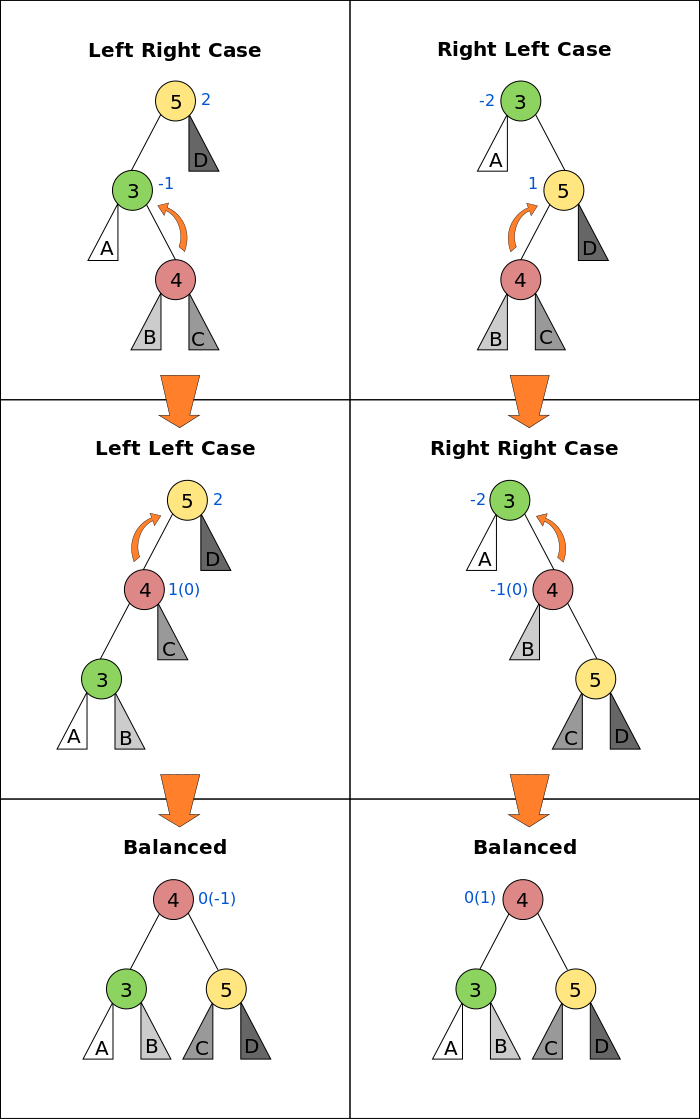
\includegraphics[width= 0.5\textwidth]{img/AVL_Tree_Rebalancing.png}
    \caption{Rebalancierung}
    \label{fig:AVL-Cases}
\end{figure}




\paragraph{Links Links / Rechts Rechts}
